\chapter{Longitudinal Evaluation of Memory, Adaptation, and Recovery}\label{ch:C27}
InMind and MemCalib distinguish two failures that an explicit-recall score can conceal. InMind probes the recognition of indirectly relevant historical information, whereas MemCalib studies whether supplied memory influences an answer too little or too strongly~\cite{inmind2026,memcalib2026}. These 2026 studies do not establish indefinite retention or reliable autonomous operation. They motivate separate interventions on admission, retrieval, interpretation, and behavioral influence, followed by longitudinal tests of changing facts, policy, and consumer versions.

Long-horizon evaluation asks whether useful behavior persists as evidence accumulates, tasks change, memory evolves, and interruptions occur. A single successful episode cannot establish this property. A system may recall explicit facts while failing to apply them indirectly, improve on one task order while regressing on another, or preserve raw history while losing authorization and temporal validity. The evaluated object is therefore a trajectory of system states rather than a sequence of independent questions.

The objective is to distinguish retention, retrieval, interpretation, influence, adaptation, and operational continuity. These mechanisms interact, but they require different controls. This chapter develops a longitudinal experimental design and connects recent memory studies to the precise claims their evidence supports.

\section{Define horizon and the unit of continuity}\label{sec:C27:horizon}
Horizon can mean model turns, tool actions, elapsed time, task count, or sessions. These quantities are correlated only under a workload model. A hundred short tool calls can be easier than a few actions separated by uncertain external events. An accelerated simulated clock can test temporal logic without establishing months-long deployment validity. Every study should declare which horizon is manipulated and which remains uncontrolled.

Continuity also has multiple units. A session can retain conversation history, a task can span several sessions, a user can have many tasks, and an organization can share a skill bank across users. The memory reset boundary determines the treatment. A fresh model call with a persistent external store is not a no-memory condition. Conversely, carrying raw conversation text without cross-session storage is not evidence of durable personal memory.

Represent a longitudinal unit by initial state, task sequence, environment-change schedule, model and harness versions, memory operations, and final outcomes. This record permits causal interventions on order, updates, and interruptions. It also exposes whether a claimed improvement is conditional on an implicit curriculum or on access to outcomes unavailable in deployment.

The two cited memory surveys provide complementary taxonomies of memory forms, functions, substrates, subjects, and dynamics~\cite{corpus251213564,corpus260206052}. Their value here is conceptual organization and discovery of primary methods. A survey's broad coverage does not independently validate the experiments it summarizes. Quantitative conclusions should return to the original method, exact version, and evaluation protocol.

The practical implication is to choose the unit of generalization before collecting runs. If the claim concerns new users, many episodes from one user do not suffice. If it concerns memory evolution, repeated calls against one fixed bank do not estimate variation in bank construction. If it concerns robustness after upgrades, a fixed-policy study cannot answer it. These distinctions determine both experimental cost and statistical uncertainty.


\section{Factor the memory pipeline}\label{sec:C27:pipeline}
A memory pipeline writes records, organizes them, retrieves candidates, selects evidence, interprets it, and influences an action. Failure at one stage can look like failure at another. If a fact was never stored, improving the reader is irrelevant. If it is stored and retrieved but ignored, improving the embedding may not help. If it is applied too strongly after becoming stale, higher recall can worsen the result.

Use staged oracle controls. Supply the original record directly to test the reader's ability to use it. Supply an oracle retrieval set to test selection and interpretation. Replace learned writing with complete raw logs to estimate extraction loss. Preserve the same action task and resource accounting. Oracle controls are diagnostic and may exceed deployable budgets, so their scores should not be presented as operational performance.

The evaluation should include negative transfer. A no-memory baseline reveals whether irrelevant or incorrect records reduce task quality. A shuffled-memory condition tests whether apparent benefit comes from generic additional text or task-specific information. A stale-memory condition tests conflict resolution. A revoked-memory condition tests authorization. These are different interventions and should not be combined into one noisy-memory score without retaining their separate outcomes.

Storage and retrieval metrics remain useful intermediate observations. Measure record coverage, provenance completeness, retrieval recall, rank quality, temporal filtering, and evidence packing. But none alone establishes useful behavior. A perfectly retrieved false record can harm the task, and a low-ranked record may be irrelevant to the action. Relate intermediate metrics to task-level outcomes through explicit ablations rather than assuming monotonic improvement.

Construction and maintenance cost belong inside the experiment. Include extraction calls, embeddings, graph updates, consolidation, deduplication, deletion, and reindexing. Report amortized cost over different reuse counts. A system that is efficient after extensive preconstruction may be unsuitable for cold-start users; another may have low initial cost but unbounded storage growth. The appropriate operating point depends on the actual longitudinal workload.


\section{Implicit relevance and appropriate influence}\label{sec:C27:influence}
InMind tests a failure mode in which a memory is relevant through a knowledge bridge rather than lexical resemblance~\cite{inmind2026}. Its paired controls distinguish storage, bridging knowledge, and query-conditioned retrieval. This is more diagnostic than asking only whether the agent can repeat a fact on demand. The benchmark is selective, however, and its authors identify domain coverage, shared answerer-judge identity, and missing negative controls against over-warning as limitations.

The mechanism suggests a concrete comparison. Hold the decisive memory and task fixed, then vary explicit recall queries, indirect application queries, direct in-context exposure, and retrieval-mediated exposure. A gap between the latter two implicates the access interface rather than necessarily the model's knowledge. To test whether a proposed remedy overuses memory, add cases where a similar stored fact should not affect the answer. Without those negatives, more frequent warning or personalization can look like better judgment.

MemCalib isolates another stage: the amount of influence a supplied memory should have~\cite{memcalib2026}. It distinguishes over-use from under-use and studies training signals that balance the two. Because the relevant memory blocks are supplied, the result concerns memory-use behavior rather than complete storage and retrieval quality. Its counterfactual localization is a credit proxy with its own uncertainty, not a direct measurement of every token's true causal contribution.

An influence evaluation needs context-dependent targets. A memory can be evidence, a preference, a constraint, or an obsolete observation. The proper response depends on provenance, current authority, and task scope. A simple rule to always prioritize memory is therefore inadequate. Test contradictory updates, exceptions, and cases where a retrieved instruction lacks authority to modify the user's objective.

These studies jointly motivate separating recall from decision use. Better retrieval can expose more relevant evidence while a poorly calibrated reader overweights it. Better memory-use training can improve interpretation while retrieval still misses implicit relevance. A complete experiment crosses retrieval policy with reader policy and reports their interaction. This factorial design can reveal whether an improvement transfers across memory engines or depends on a particular writer-reader pairing.


\section{Task order adaptation and hidden curricula}\label{sec:C27:order}
An evolving memory makes task order part of the treatment. Early episodes determine which procedures and mistakes enter the bank; later episodes determine whether those records are useful. A default dataset order may contain an implicit curriculum, grouping related tasks or increasing difficulty. Improvement along that sequence does not establish order-robust learning.

The fragility study reevaluates memory-based self-improving agents across multiple runs and shuffled orders, identifying substantial sensitivity to variance, order, and underspecification~\cite{ye2026fragility}. Its findings apply to the tested methods and environments, not every possible self-improvement architecture. The methodological implication is strong: one cumulative curve under one order is insufficient evidence for a stable improvement mechanism.

Use several independently constructed memory trajectories for each experimental condition. Within a trajectory, tasks share an evolving bank and are dependent. Across trajectories, randomize order and model sampling as declared. If a common initial bank is used, treat its construction as another factor rather than assume it is representative. Report variation across banks and orders, not only average task accuracy pooled over all calls.

Curriculum effects can be studied directly. Compare random order, grouped order, reversed order, and an explicitly designed curriculum while holding the task multiset fixed. A curriculum that improves performance is a legitimate result if named as such. The error is presenting that conditional benefit as spontaneous general improvement. Also test new task families that do not share the procedures learned early in the sequence.

Underspecified tasks can contaminate memory with misleading lessons. If a failure arose from an ambiguous objective or unavailable tool, the agent may store an incorrect procedural correction. Later reuse then amplifies the original ambiguity. Memory construction should record failure attribution and uncertainty, and evaluations should distinguish environment failure from policy failure. Additional rubrics can improve specification while also giving the learner more supervision; that information difference belongs in the treatment description.


\section{Temporal change deletion and migration}\label{sec:C27:change}
A persistent memory must cope with facts becoming false, permissions changing, and representations drifting. Static recall benchmarks cannot test these transitions. A useful longitudinal suite includes explicit corrections, contradictory sources of unequal authority, expired preferences, deletion requests, user separation, and model or embedding upgrades. The required behavior is not always to retain more: sometimes it is to stop using a previously useful record.

Define the validity interval of a fact separately from its observation timestamp. A record can remain historically true while becoming inapplicable to the current decision. Retrieval should expose this distinction, and the reader should not treat a recent ingestion time as evidence of recent event time. Inject delayed reports and backdated corrections to test whether the system confuses the two.

Deletion tests must follow derivatives. Raw events can generate summaries, embeddings, graph edges, skills, caches, and copied subagent context. Removing one row does not establish complete erasure. A test should enumerate the lineage, verify retrieval exclusion, and check whether reconstruction can reintroduce deleted content. Physical deletion, logical exclusion, and retention under restricted audit policy are different outcomes.

Migration changes memory meaning. A new embedding model can alter nearest neighbors; a new policy can interpret the same skill differently; a schema conversion can drop provenance or confidence. Compare pre- and post-migration behavior on held-out tasks and known conflict cases. A successful database migration does not establish behavioral compatibility. Retain the old representation where permitted so failures can be traced and rollback can be assessed.

Authorization is particularly sensitive to restored state. A checkpoint can contain a historical grant, but a resumed session must consult current authority. The experiment should revoke access while the task is paused and then resume from the old checkpoint. Measure whether the forbidden record remains in model-visible context and whether new effects are blocked. This tests context-memory-policy consistency rather than storage persistence alone.


\section{Horizon-dependent reliability and survival}\label{sec:C27:survival}
Long tasks can be analyzed through time to a defined failure event. Let $T$ be the first step at which a required invariant is violated and $S(h)=\Pr(T>h)$ the survival probability through horizon $h$. The hazard at step $t$ is $\lambda_t=\Pr(T=t\mid T\geq t)$. Then $S(h)=\prod_{t=1}^{h}(1-\lambda_t)$ under the corresponding discrete-time definitions. Here $T\in\mathbb N_{>0}\cup\{\infty\}$, $h\in\mathbb N_0$, the empty product is one, and $\lambda_t$ is defined only while $\Pr(T\geq t)>0$. The identity does not assume a constant hazard.

This representation distinguishes cumulative exposure from worsening policy. A system with constant small per-step risk can have declining long-horizon success without becoming less competent at each step. Conversely, memory contamination or context loss can make the hazard increase over time. Stratify failures by cause and inspect their relationship to compaction, retrieval, updates, and interruptions. A single final completion rate cannot distinguish these explanations.

Censoring requires care. If a run ends because the budget expires before failure or completion, the censoring mechanism may depend on task difficulty. Standard survival estimators require assumptions about that dependence. Report budget exhaustion explicitly and avoid treating censored trajectories as successful survivors indefinitely. Competing events, such as authorization failure, evaluator outage, and task completion, may require cause-specific analysis rather than one undifferentiated stopping time.

In particular, successful completion removes a run from exposure to further task actions. To distinguish this event from failure, let $U$ be the first absorbing stopping time under the study protocol and $J$ its cause. For each cause $j$, define $\lambda_j(t)=\Pr(U=t,J=j\mid U\geq t)$ while the risk set is nonempty. Then
\begin{equation}
 S_U(h)=\prod_{t=1}^{h}\left(1-\sum_j\lambda_j(t)\right),\qquad
 F_j(h)=\sum_{t=1}^{h}S_U(t-1)\lambda_j(t).
\end{equation}
Here the causes are mutually exclusive, $\sum_j\lambda_j(t)\leq1$, and $F_j(h)=\Pr(U\leq h,J=j)$ is the cumulative incidence of that stopping cause. Treating completed tasks as ordinary independent censoring can instead estimate a hypothetical continued-exposure process. Faster completion and lower failure hazard are different interventions; report completion incidence, failure incidence, and unresolved budget stops separately. The identity is a probability decomposition, not a claim that a particular survival estimator is justified for the available logs.

Recovery changes the event definition. A transient tool failure that is correctly reconciled may not count as task failure, while an undetected duplicate effect may violate an invariant even if the final artifact looks correct. Declare whether the study measures first fault, unrecovered fault, constraint violation, or final failure. Each is useful, but they answer different operational questions.

Uncertainty should cluster by longitudinal unit, not by step. Thousands of steps from one evolving bank do not provide thousands of independent observations about population reliability. Report the number of independent users, sessions, task streams, and bank constructions. Where the data are limited, present the observed trajectories and conditional conclusions rather than fitting an elaborate hazard model whose parameters are weakly identified.


\section{A longitudinal implementation and reporting contract}\label{sec:C27:implementation}
The evaluator needs a clock, task scheduler, environment-change injector, memory snapshotter, and artifact verifier. These components should be separate from the agent's own tools. Otherwise the agent can observe future tasks, change the evaluation clock, or inspect outcomes intended only for grading. A simulated environment can provide controlled interventions, but its simplifications must be identified when generalizing to deployment.

For every memory operation, record writer identity, source event, model and harness version, record type, validity scope, permissions, and affected derivatives. Read operations should record candidate sets and selected evidence where feasible. This enables failure attribution: a missing fact, bad ranking, inappropriate influence, and stale authorization leave different traces. Privacy constraints may limit released content, but event structure and redaction policy can still be documented.

The baseline set should include no memory, raw-log retrieval, simple lexical or dense retrieval, curated factual records, procedural memory, and an oracle evidence condition. Match task streams and budgets, and include construction cost. A complex system should demonstrate benefit over a strong simple baseline, not only over an intentionally weak store. Report where simpler methods win and whether the difference survives shuffled orders.

The October 2026 audit of MemoryAgentBench's conflict-resolution split supplies a more specific baseline: a frozen parser and last-write resolver that directly executes the benchmark's newest-statement rule~\cite{pakhomov2026gold}. The parser was developed on one fact list and held fixed on three others. The audit separates parser or path-composition residuals from items whose released answer is unreachable in its frozen parser's final last-write graph. This operational classification does not itself prove that the released label is wrong: a fuller parser or a different grounding rule can change reachability. Its principal item-level model comparisons retain one scored outcome per item, without mechanism traces, and do not run learned or structured memory systems. Thus an apparent failure can reflect a label--rule conflict, rather than evidence that an agent failed selective forgetting; the audit does not establish how a particular memory mechanism reasons internally.

This case changes the experimental unit. Hundreds of questions sharing four fact lists do not constitute hundreds of independent histories. Answer-level uncertainty is conditional on those lists; generalization across history construction is limited by the small number of distinct streams. A proposed extension generates independent update streams from a versioned state machine, derives answers by replay, and verifies the gold graph independently of the agent's parser. Include first-write, last-write, valid-time, and authority-aware resolvers as distinct baselines only where the task semantics warrant them. Blindly applying last-write order to real organizational evidence would be incorrect when a later source has lower authority or reports an earlier valid-time interval. Benchmark-rule correctness and deployment conflict semantics must remain separate.

HyperSkill's sequential fixed-order evaluation, extra LLM maintenance calls, and gold-outcome main setting illustrate why these fields matter~\cite{xu2026hyperskill}. Its structured memory mechanism is substantive, while concurrency, order robustness, and deployment feedback availability require additional evidence. Similarly, context-management results that retain raw offloaded history should not be interpreted as indefinite usable memory without testing retrieval and decision preservation~\cite{corpus260723809}.

The practical output is a trajectory-level evidence record that supports both mechanism analysis and operational decisions. It should show what the system retained, what it retrieved, how it used the evidence, what changed, and which constraints survived. This is a more demanding standard than a recall score, but it is necessary when memory is expected to influence long-running agents across users, tasks, and versions.

\section{A counterfactual session-stream experiment}\label{sec:C27:streamcase}
Consider a technical assistant supporting a software team over a sequence of repository tasks. Early sessions establish that one service uses a particular deployment command, that production changes require review, and that a diagnostic document belongs to a restricted project. Later sessions change the command, introduce an exception for a sandbox environment, revoke one user's access, and ask an indirect question whose answer depends on the old experience. The test is not whether the assistant can repeat each fact. It is whether it uses the correct record, scope and authority when choosing an action.

Construct independent task streams from templates with controlled entity substitutions, dependency structures and change schedules. The substitutions prevent exact-string memorization from explaining transfer, while the dependency structure preserves the reasoning required. Separate streams should not share answer-bearing memory unless cross-user sharing is explicitly the treatment. The evaluator retains the authoritative event sequence and can query the environment, but the agent sees only observations available at each step.

Table~\ref{tab:C27:interventions} lists interventions that distinguish the relevant mechanisms. Each row specifies what changes and what observation would diagnose the failure. The table is an experimental design, not a set of reported measurements.
\begingroup\setlength{\tabcolsep}{3pt}\small
\begin{longtable}{L{23mm}L{40mm}L{45mm}}
\caption{Counterfactual interventions in a session stream.}\label{tab:C27:interventions}\\
\toprule Intervention & Controlled change & Diagnostic observation \\
\midrule\endfirsthead
\toprule Intervention & Controlled change & Diagnostic observation \\
\midrule\endhead
Write omission & Remove one source event from the writer input. & A missing record should be attributed to acquisition or writing, not retrieval. \\
Oracle record & Supply the decisive record directly in context. & Continued failure implicates interpretation or action policy under this control. \\
Implicit query & Replace explicit recall wording with a knowledge bridge. & A direct-versus-indirect gap identifies a relevance-routing limitation. \\
Contradiction & Add a newer authoritative correction. & The selected record and action should reflect validity and authority, not mere recency. \\
Scope exception & Make an old procedure valid only in a sandbox. & Blanket reuse or blanket rejection reveals inadequate applicability reasoning. \\
Revocation & Remove a principal's access while paused. & Resumption must not turn historical access into a new authorized effect. \\
Deletion & Remove source content and mark derivatives. & Retrieval and reconstruction should not silently reintroduce excluded information. \\
Migration & Change policy or embedding version at a boundary. & Differences should be linked to representation, retrieval or interpretation changes. \\
\bottomrule\end{longtable}
\endgroup

The baseline conditions should preserve information and budget as carefully as possible. A direct-context oracle can consume more prompt space than a retrieval system, so reserve equivalent context capacity or report the difference. A full-history baseline can become infeasible at long horizons; report the horizon at which it ceases to fit rather than silently switching its truncation policy. A simple raw-log retriever provides an important control because it avoids extraction errors while retaining the same source evidence.

Writer and reader policies should be crossed. A high-quality writer paired with a weak reader may produce accurate records that are misapplied. A strong reader paired with an aggressive summarizer may never receive the decisive constraint. Crossing these components identifies interaction effects and prevents a memory engine from receiving credit for a better backbone. The experiment should also vary whether outcome feedback is gold, self-judged, delayed or unavailable. A method that relies on immediate correct labels has a different deployment requirement from one operating without them.

Task order needs independent replication. Generate several permutations of the same multiset and several independently sampled streams. The first comparison isolates curriculum effects conditional on the tasks; the second supports broader generalization. Preserve the entire evolving memory for each run so failures can be traced to prior updates. Reusing a bank built under one order across all conditions would remove an important source of variation and could favor methods compatible with that bank's organization.

The primary outcomes include verified task completion, constraint adherence, temporal correctness, authorized evidence use and recovery after interruption. Intermediate outcomes include write coverage, retrieval of decisive records, correct rejection of obsolete records and calibrated influence. These outcomes should be linked rather than pooled indiscriminately. For example, a retrieval improvement with no action improvement can reveal a reader bottleneck; an action gain accompanied by unauthorized context use is not an acceptable solution to the stated task.

Negative controls are essential. Include tasks where the remembered deployment command is irrelevant, where the restricted document is unnecessary, and where the sandbox exception should not generalize. Otherwise an agent that always emits warnings or always retrieves every memory can receive undeserved credit. Measure over-application and under-application separately, as motivated by MemCalib, while retaining the end-to-end storage and retrieval components that its supplied-memory setting intentionally isolates.

Failure adjudication should use the event history and artifact state, not the agent's explanation alone. A stored memory can claim that a tool failed because credentials were invalid when the actual cause was a temporary outage. If this explanation becomes a procedural rule, later tasks may avoid a useful tool unnecessarily. The evaluator should identify the original observation, the inferred lesson and the later consequence. This causal chain distinguishes bad experience attribution from simple forgetting.

Finally, report the maintenance workload as the bank grows. Track raw and derived storage, index updates, compaction, merge operations, deletion propagation and retrieval latency. A sublinear skill count does not imply bounded total memory if raw trajectories and subtask nodes continue to grow. Nor does a compact bank guarantee low decision cost if each query invokes extensive reasoning. The study should expose which resource grows with episodes, which is amortized across reuse, and which can be bounded only by discarding information. Those operating conditions determine whether a promising memory mechanism can support sustained agent execution.

The public HyperSkill implementation provides a concrete separation between the hypergraph core and the per-task provider interface\cite{xu2026hyperskill}. A reproduction should instrument both: the core determines candidate reachability and maintenance, while the provider determines when retrieval and ingestion occur relative to task execution. Logging only final skill counts would miss a provider that ingests outcome information too early. Logging only model context would miss a maintenance operation that changes the interpretation of later records. Attach task and memory-version identifiers to each operation so the two traces can be joined.

The implementation audit should also verify that the evaluator's gold outcome is unavailable to deployment-style variants before they commit their own interpretation. A gold-feedback experiment is useful for estimating mechanism potential, but it should not be confused with a self-judged agent. When switching to self-judgment, measure the resulting memory-label errors and their downstream accumulation rather than reporting only final success. A modest immediate error rate can have a disproportionate longitudinal effect if the same mistaken lesson is reused repeatedly.

The fragility study's published code and InMind's released diagnostic resources offer additional primary anchors for this audit\cite{ye2026fragility,inmind2026}. Their existence improves inspectability but does not establish that the experiment described here has run. The appropriate next record is an immutable implementation revision, complete stream manifest and trace of the actual interventions. Until those observations exist, the proposed factorial and counterfactual tests remain a research design with explicit rejection criteria, not evidence of achieved lifelong reliability.

The inspected provider exposes \path{provide_memory} and \path{take_in_memory}; instrumentation at these boundaries can establish whether evidence was supplied before a decision or incorporated only after the task outcome.

\subsection{What a counterfactual replay can identify}\label{sec:C27:counterfactualreplay}
Replaying logged actions under a changed memory policy does not by itself estimate that policy's end-to-end performance. Once a changed context induces another action, the future tool results, environment and memory writes can diverge. Continuing to supply the original observations then evaluates a hybrid trajectory that neither policy would necessarily generate. The problem is particularly acute for recoverable effects: an original successful write cannot be assumed to exist after a counterfactual policy chose a read instead.

A frozen-prefix test can legitimately compare next-action distributions from the same recorded state, provided both contexts contain only information available at that boundary. This identifies local sensitivity, such as whether a revoked instruction changes a proposal, rather than full task success. A full counterfactual test must rerun the environment from a valid checkpoint or use a justified transition model, exposing model error and replay limits. Importance weighting requires logged behavior probabilities and support for the alternative actions; deterministic tool logs do not supply those conditions automatically. Thus paired prefix diagnostics, complete reruns and model-based counterfactuals should be reported as distinct evidence products rather than interchangeable forms of replay.


Figure~\ref{fig:C27:overview} isolates the mechanism and its stated information boundaries.
\begin{figure}[!htbp]
\centering
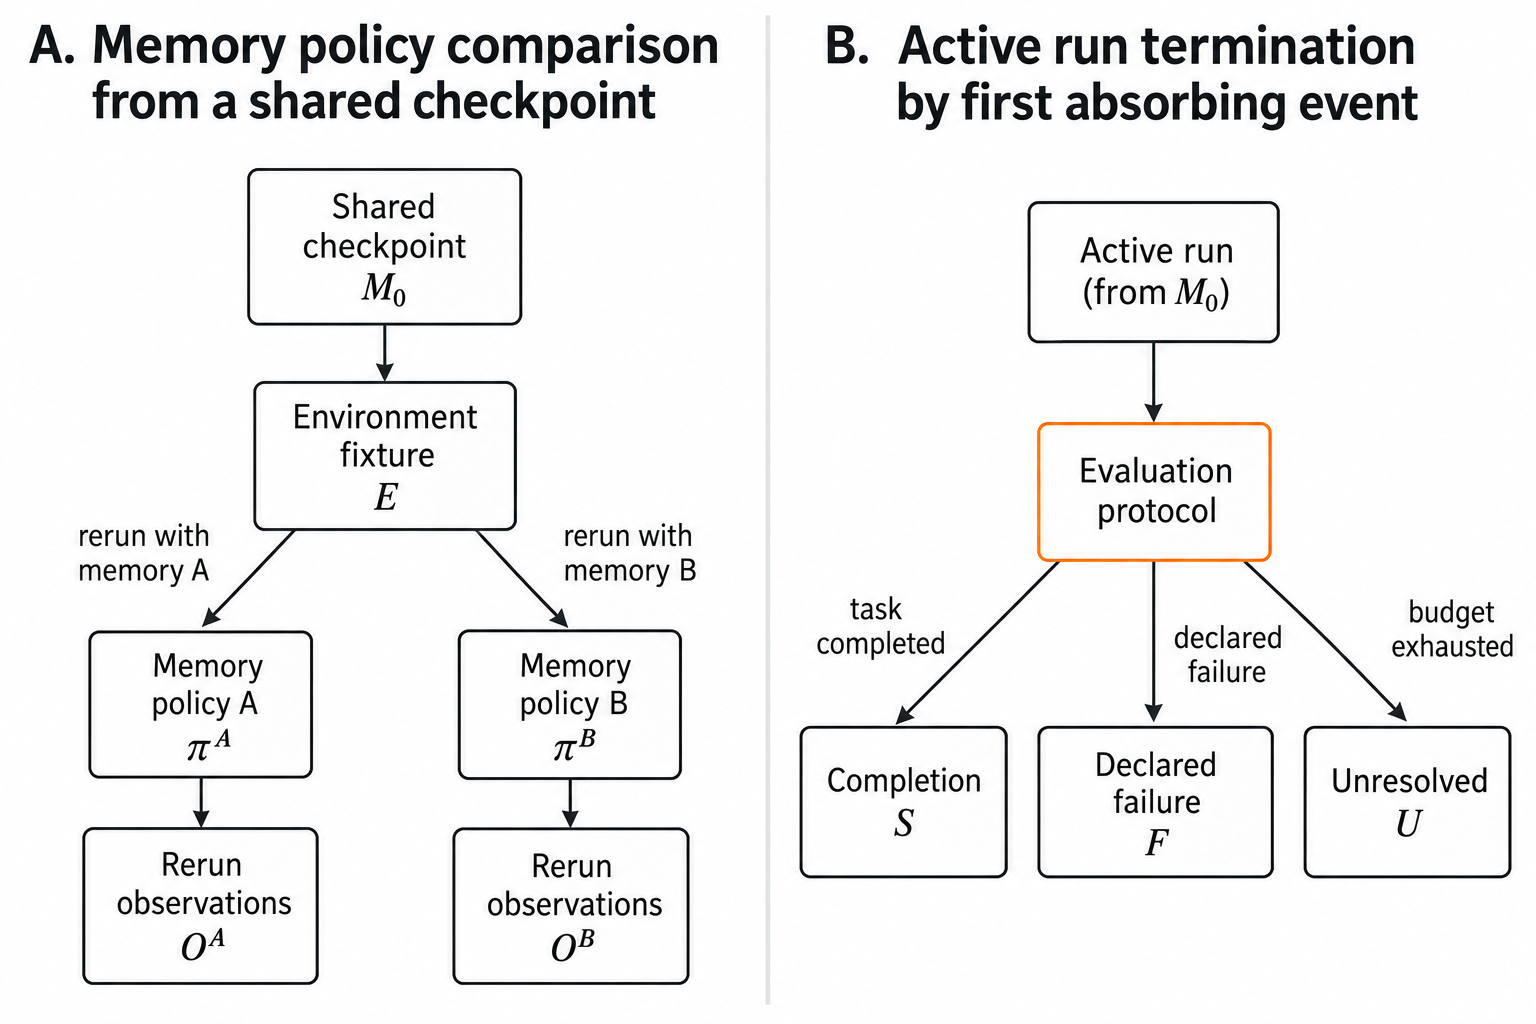
\includegraphics[width=\linewidth]{book/figures/assets/F27review.png}
\caption{Memory policies $\pi^A,\pi^B$ share an initial fixture $(M_0,E)$ but can produce different rerun observations $O^A,O^B$. Observation-changing counterfactuals require valid reruns, not substituted answers on one fixed log. Completion $S$, declared failure $F$ and unresolved budget stops $U$ are distinct protocol outcomes; interpreting a stop as censoring requires additional assumptions. The figure-local S/F/U labels name outcome categories, not stopping times.}
\label{fig:C27:overview}
\end{figure}

